\section{Deployment constraints}
\label{sec:limits}

\paragraph{Batching and concurrency.}
AR-30B improves throughput by \arBatchMult$\times$ in its batching
experiment, whereas DG reaches up to $1.7\times$ in the tested
configurations. LLaDA-8B on the dInfer inference engine reaches approximately $1.2\times$.
The diffusion measurements are implementation-limited: the tested vLLM
path restricts mixed-phase batches, and dInfer was run without its
intended cache. They establish modest gains on those stacks, not an
upper bound on diffusion batching.

\begin{figure}[ht!]
\centering
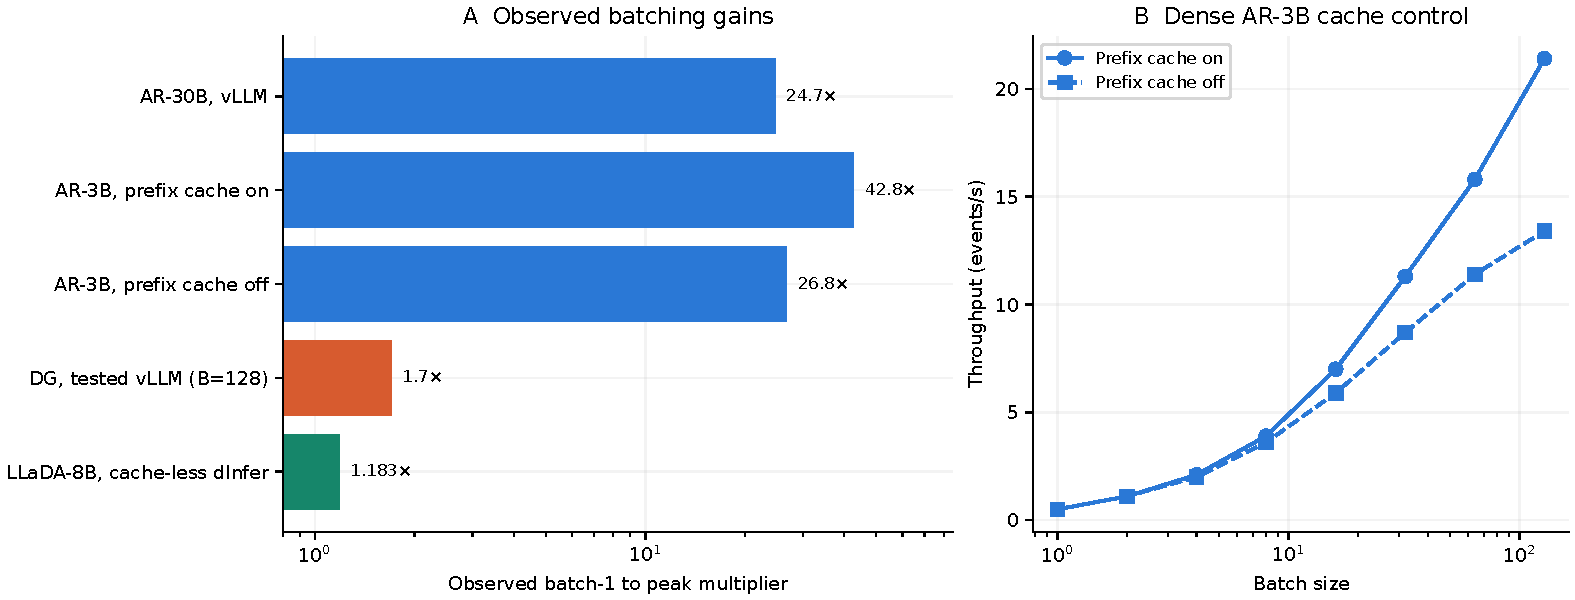
\includegraphics[width=\linewidth]{figures/fig6_batching.pdf}
\caption{Observed throughput multipliers for several model/runtime pairs.
The primary AR-30B result is approximately $25\times$. The cache-on/off
control uses dense AR-3B. Disabling cross-request
prefix caching lowers that model's multiplier from \cacheOnMult$\times$
to \cacheOffMult$\times$, so shared prefixes alone do not explain
its throughput gain. These controls do not identify a universal DG limit.}
\label{fig:batching}
\end{figure}

Sequential steps within one request chain cannot batch with each other,
but requests from independent chains can still overlap. Likewise,
interactivity and tenant isolation do not necessarily require a dedicated
batch-1 GPU. Deployment decisions should use measured arrival patterns,
scheduler behavior, and latency targets. Appendix~\ref{app:batching}
separates the cache observations from possible explanations.

\paragraph{Absolute and relative tails.}
In the repeated primary-pair measurements, AR-30B has CV
\arThirtyCV\% and max/median $1.75\times$, compared with
\dgThirtyCV\% and $3.07\times$ for DG. However, DG's absolute
p99 is \dgPninetyNine\,ms versus AR's \arPninetyNine\,ms.
A larger relative tail does not imply a slower absolute response or
a service-level agreement (SLA) violation. The relevant test is the specified latency percentile
under the intended arrival process. Sample maxima are not worst-case
bounds, and comparing maximum ratios across unequal sample sizes is
particularly fragile (Appendix~\ref{app:distributions}).

\paragraph{Prompt length and decoding settings.}
Longer prompts increase DG cost and can move the fitted crossover.
The input-slope comparison uses dense AR-3B and cannot be transferred
numerically to AR-30B. Canvas size and $K$ also change both cost and
quality. A joint sweep finds a better measured operating point than the
paper's reference setting: canvas 128, $K{=}8$ gives 368\,ms and
F1 0.864 versus 376\,ms and 0.853 at canvas 256, $K{=}8$.
These are point estimates on one sample, not a statistically established
improvement for all workloads (Appendix~\ref{app:input_canvas}).

\paragraph{Memory and co-residency.}
The nominal 52--60\,GB bf16 weight footprints of the primary pair
leave limited space for other large models on an 80\,GB GPU. Actual
capacity also depends on KV caches, activations, and runtime allocations.
A dense AR-1.5B has much smaller weights, but dividing GPU memory by
weight size cannot establish how many serving replicas fit or how their
throughput scales. We have not measured concurrent replicas, contention,
or isolation overhead, and make no linear co-residency speedup claim.

\paragraph{Cost accounting.}
At an assumed GPU rental rate $r$ dollars/hour, mean service time
$\bar t$ seconds/event, and busy fraction $u$, a simple single-instance
allocation is
\begin{equation}
 c_{\mathrm{event}}=\frac{r\bar t}{3600u}.
\end{equation}
This assumes the same GPU is rented throughout both busy and idle periods;
it excludes central processor, storage, networking, and retry costs. At fixed demand,
lower latency does not reduce the bill for an always-on GPU unless it
allows fewer provisioned resources or more useful work. A latency-based rental estimate therefore does not establish realized
annual savings. Batching economics should use measured throughput and
the quality requirement, rather than a serial latency ratio alone.

For a deadline-bound task, first establish which configurations return
acceptable records on time, then compare their costs. A configuration
that processes more records per second may still deliver each record too
late for that task. Conversely, the serial comparison does not show that
every AR configuration misses the target: scheduler, model, and decoding
choices require measurement at the intended load.
